\documentclass[12pt]{article}
\usepackage[utf8]{inputenc} % Ensure proper encoding
\usepackage{amsmath, amssymb}
\usepackage{geometry}
\geometry{a4paper, margin=1in}
\usepackage{enumitem}
\usepackage{hyperref}
\usepackage{graphicx}
\usepackage{caption}
\usepackage{listings}
\usepackage{xcolor}

% Define code listing style
\lstset{
    language=Python,
    basicstyle=\ttfamily\small,
    keywordstyle=\color{blue},
    stringstyle=\color{red},
    commentstyle=\color{green!50!black},
    numbers=left,
    numberstyle=\tiny,
    stepnumber=1,
    numbersep=5pt,
    showspaces=false,
    showstringspaces=false,
    frame=single,
    breaklines=true,
    breakatwhitespace=true,
    tabsize=4
}

\title{The Role of Linear Regression in the Kalman Filter System: A Comprehensive Analysis with Simulated Data}
\author{Gary Hobson \\ Southern New Hampshire University \\ MAT 300}
\date{\today}
%\date{April 04, 2025}

\begin{document}

\maketitle

\begin{abstract}
This report provides an in-depth analysis of how linear regression can be integrated into the Kalman filter framework to estimate the state transition model for dynamic systems. The Kalman filter, a recursive state estimation algorithm, relies on an accurate state transition matrix to predict system states, but this matrix is often unknown or approximate in real-world applications. Linear regression offers a data-driven approach to learn this matrix from noisy observations, enhancing the filter’s adaptability. Through a simulated one-dimensional vehicle system observed by GPS and Lidar sensors, we demonstrate the effectiveness of regression in modeling state dynamics. The analysis includes detailed mathematical derivations, regression diagnostics, a nested F-test, practical applications, and comparisons with theoretical models. This report aims to provide a thorough understanding of this integration, suitable for academic and practical exploration in statistical state estimation.
\end{abstract}
%\maketitle
\newpage

\tableofcontents
\clearpage

\section{Introduction}
\label{sec:intro}

State estimation is a critical process in science and engineering, allowing us to infer the condition of dynamic systems—like a vehicle’s position or a stock’s volatility—from noisy, incomplete data. The Kalman filter, a recursive algorithm introduced in 1960 by Rudolf E. Kalman, is a cornerstone of this field. It excels at optimally combining predictions with observations under linear and Gaussian assumptions, finding applications in GPS navigation, robotics, and financial modeling. The filter operates in two phases: the \textit{prediction step}, which forecasts the next state using a state transition model, and the \textit{update step}, which refines this forecast with new measurements.

The state transition model, often a matrix derived from physical laws (e.g., kinematic equations), is vital to the prediction step’s accuracy. However, in practice, this model may be unknown or imprecise due to unmodeled dynamics or environmental factors. This project investigates how linear regression can estimate the state transition model from data, enhancing the Kalman filter’s predictive power in a data-driven context.

For this MAT 300 final project, I simulate a one-dimensional dynamic system—a vehicle moving along a straight path—with state variables of position (\( p_t \)) and velocity (\( v_t \)), observed by GPS and Lidar sensors. These sensors introduce noise and bias, reflecting real-world challenges. The dataset includes time (\( t \)), current position (\( p_t \)), velocity (\( v_t \)), sensor type (\( S \): 0 = GPS, 1 = Lidar), and next position (\( p_{t+1} \)) as the response variable. Using Python, I generate 200 time steps of simulated data, adding controlled noise to mimic sensor imperfections.

My approach involves building a first-order main effects regression model to predict \( p_{t+1} \) from \( p_t \), \( v_t \), and \( S \), followed by a model with interaction terms to explore sensor-specific effects. I will assess model fit using regression diagnostics (e.g., residual analysis, multicollinearity checks) and perform a nested F-test to compare the models. Beyond diagnostics, I evaluate predictive accuracy with mean squared error (MSE). I hypothesize that the interaction model will better capture system dynamics, improving position estimates by accounting for sensor differences.


\section{Background on the Kalman Filter}
\label{sec:background}

\subsection{Historical Context}
\label{subsec:historical_context}

The Kalman filter emerged during a pivotal period in control theory and signal processing. In 1960, Rudolf E. Kalman, then at the Research Institute for Advanced Study in Baltimore, published his groundbreaking paper \textit{``A New Approach to Linear Filtering and Prediction Problems''} \cite{kalman1960}, which introduced a new approach to linear filtering and prediction. Building on Norbert Wiener’s earlier work on stationary time-series prediction \cite{wiener1949}, Kalman addressed several limitations of Wiener’s method, including its restriction to stationary statistics and infinite memory filters. As Kalman notes, “The classical filtering and prediction problem is re-examined using the Bode-Shannon process, and the ‘state transition’ method of analysis of dynamic systems” \cite{kalman1960}. This state-space approach allowed the Kalman filter to handle both stationary and nonstationary systems, making it suitable for real-time applications like aerospace navigation during the Space Race.

Kalman’s innovation was particularly timely given the technological demands of the era. The 1960s saw rapid advancements in aerospace engineering, driven by the need for precise navigation and control in space missions. The Kalman filter’s ability to provide optimal state estimates in the presence of noise made it a critical tool for projects like the Apollo program, where it was used to navigate spacecraft to the moon. Its recursive nature—updating estimates with each new measurement without requiring the entire history of data—further enhanced its practicality for real-time systems with limited computational resources.

The significance of Kalman’s contribution is evident in its enduring relevance. Pei et al. \cite{pei2019} highlight its modern applications: “Kalman filtering is a state estimation technique invented in 1960 by Rudolf E. Kálmán… used in many application areas including spacecraft navigation, motion planning in robotics, signal processing, and wireless sensor networks” \cite{pei2019}. The filter’s adaptability to diverse domains underscores its importance, and this report leverages linear regression to further enhance its flexibility by estimating system dynamics from data.

The historical context also highlights the evolution of state estimation techniques. Wiener’s approach, while groundbreaking, was limited by its assumptions of stationarity and the need for infinite memory, making it impractical for systems with time-varying dynamics or limited computational power. Kalman’s state-space formulation overcame these limitations by representing the system in terms of its state vector and transition dynamics, allowing for a more general and computationally efficient solution. This shift paved the way for modern extensions like the Extended Kalman Filter (EKF) and Unscented Kalman Filter (UKF), which address non-linear systems, as discussed later in this report.

\subsection{Mathematical Framework}
\label{subsec:math_framework}

For a discrete-time linear system, the state vector \( \mathbf{x}_t \in \mathbb{R}^n \) evolves according to:

\begin{equation}
    \mathbf{x}_{t+1} = F \mathbf{x}_t + \mathbf{w}_t,
    \label{eq:state_transition}
\end{equation}

where:
\begin{itemize}
    \item \( F \in \mathbb{R}^{n \times n} \) is the state transition matrix,
    \item \( \mathbf{w}_t \sim N(0, Q) \) is Gaussian process noise with covariance \( Q \).
\end{itemize}

Measurements \( \mathbf{z}_t \in \mathbb{R}^m \) are given by:

\begin{equation}
    \mathbf{z}_t = H \mathbf{x}_t + \mathbf{v}_t,
    \label{eq:measurement}
\end{equation}

where:
\begin{itemize}
    \item \( H \in \mathbb{R}^{m \times n} \) is the observation matrix,
    \item \( \mathbf{v}_t \sim N(0, R) \) is measurement noise with covariance \( R \).
\end{itemize}

The Kalman filter iterates through two steps:

\textbf{Prediction Step:}
\begin{itemize}
    \item Predicted state: \( \hat{\mathbf{x}}_{t+1|t} = F \hat{\mathbf{x}}_{t|t} \),
    \item Predicted covariance: \( P_{t+1|t} = F P_{t|t} F^T + Q \).
\end{itemize}

\textbf{Update Step:}
\begin{itemize}
    \item Kalman gain: \( K_{t+1} = P_{t+1|t} H^T (H P_{t+1|t} H^T + R)^{-1} \),
    \item Updated state: \( \hat{\mathbf{x}}_{t+1|t+1} = \hat{\mathbf{x}}_{t+1|t} + K_{t+1} (\mathbf{z}_{t+1} - H \hat{\mathbf{x}}_{t+1|t}) \),
    \item Updated covariance: \( P_{t+1|t+1} = (I - K_{t+1} H) P_{t+1|t} \).
\end{itemize}

The state transition matrix \( F \) is central to the prediction step. For a system with position \( p_t \) and velocity \( v_t \), \( \mathbf{x}_t = [p_t, v_t]^T \), and:

\begin{equation}
    F = \begin{bmatrix} 1 & \Delta t \\ 0 & 1 \end{bmatrix},
    \label{eq:ideal_F}
\end{equation}

implying \( p_{t+1} = p_t + v_t \cdot \Delta t \), \( v_{t+1} = v_t \). This matrix assumes constant velocity and linear motion, a common model in kinematics. However, in practice, \( F \) may be affected by unmodeled dynamics (e.g., acceleration, friction) or external factors (e.g., wind, sensor bias), necessitating estimation from data.

To derive the Kalman gain, consider the update step in more detail. The innovation \( \mathbf{z}_{t+1} - H \hat{\mathbf{x}}_{t+1|t} \) represents the difference between the actual measurement and the predicted measurement. The Kalman gain \( K_{t+1} \) weights this innovation to minimize the mean squared error of the state estimate, balancing the uncertainty in the prediction (\( P_{t+1|t} \)) and the measurement noise (\( R \)). The updated covariance \( P_{t+1|t+1} \) reflects the reduced uncertainty after incorporating the measurement, ensuring the filter remains optimal over time.

The optimality of the Kalman filter relies on the assumptions of linearity and Gaussian noise. For a linear system with Gaussian noise, the filter provides the minimum mean squared error (MMSE) estimate of the state, as proven by Kalman \cite{kalman1960}. This property makes it particularly effective for systems where these assumptions hold, but it also highlights the need for accurate models of \( F \), \( Q \), and \( R \). When \( F \) is uncertain, linear regression can estimate it from data, as explored in this report.

\section{Simulation of the Dynamic System}
\label{sec:simulation}

\subsection{System Design}
\label{subsec:system_design}

I will simulate a one-dimensional dynamic system representing a vehicle moving along a straight path. The state vector is \( \mathbf{x}_t = [p_t, v_t]^T \), where:
\begin{itemize}
    \item \( p_t \): Position (meters),
    \item \( v_t \): Velocity (meters/second).
\end{itemize}

The true dynamics are:

\begin{align}
    p_{t+1} &= p_t + v_t \cdot \Delta t + w_t, \label{eq:sim_position} \\
    v_{t+1} &= v_t + u_t, \label{eq:sim_velocity}
\end{align}

where:
\begin{itemize}
    \item \( \Delta t = 1 \) second,
    \item \( w_t \sim N(0, 0.1) \) is process noise for position,
    \item \( u_t \sim N(0, 0.05) \) is process noise for velocity.
\end{itemize}

These noise levels simulate small perturbations from factors like wind, friction, or sensor drift, typical in physical systems. The choice of \( \Delta t = 1 \) simplifies the dynamics, making the state transition matrix:

\begin{equation}
    F = \begin{bmatrix} 1 & 1 \\ 0 & 1 \end{bmatrix},
    \label{eq:sim_F}
\end{equation}

but I will estimate this matrix using regression to account for noise and potential deviations from the ideal model.

The system design reflects a simplified kinematic model, assuming constant velocity between time steps. In reality, vehicles may experience acceleration, braking, or external forces (e.g., gravity on a slope). By introducing process noise, we simulate these unmodeled effects, making the system more representative of real-world scenarios. The noise variances (0.1 for position, 0.05 for velocity) were chosen to balance realism and challenge, ensuring the regression task is non-trivial but feasible.

\subsection{Sensor Models}
\label{subsec:sensor_models}

Two sensors observe the position:
\begin{itemize}
    \item \textbf{GPS}: \( z_t = p_t + v_t \), \( v_t \sim N(0, 0.5) \). GPS is unbiased but noisy, reflecting atmospheric interference, satellite geometry, or multipath effects.
    \item \textbf{Lidar}: \( z_t = p_t + 0.2 + v_t \), \( v_t \sim N(0.2, 0.3) \). Lidar is precise but biased by 0.2 meters, mimicking calibration errors or misalignment.
\end{itemize}

The noise and bias parameters were chosen to reflect real-world sensor characteristics:
\begin{itemize}
    \item GPS noise (\( \sigma = 0.5 \)) captures its lower precision, typical of consumer-grade GPS receivers with errors of 5-10 meters.
    \item Lidar’s smaller noise (\( \sigma = 0.3 \)) and bias (0.2 meters) emulate its higher accuracy (often within centimeters) but potential systematic offsets due to improper calibration or environmental factors (e.g., reflective surfaces).
\end{itemize}

This dual-sensor setup tests regression’s ability to model the state transition despite varying noise and bias, and to determine whether sensor type influences the dynamics beyond the measurement process.

\subsection{Data Generation}
\label{subsec:data_generation}

Starting with \( p_0 = 0 \), \( v_0 = 1 \), we generated 200 time steps, randomly assigning GPS or Lidar at each step (50\% probability). The dataset includes:
\begin{itemize}
    \item Time (\( t \)),
    \item Current position (\( p_t \)),
    \item Velocity (\( v_t \)),
    \item Sensor type (\( S \): 0 = GPS, 1 = Lidar),
    \item Next position (\( p_{t+1} \)).
\end{itemize}

The initial conditions (\( p_0 = 0 \), \( v_0 = 1 \)) simulate a vehicle starting from rest with a constant velocity. The random assignment of sensors ensures a balanced dataset, allowing us to assess sensor-specific effects without bias toward one sensor type. The 200 time steps provide sufficient data for regression while keeping computational demands manageable.

To generate the data, we iteratively applied the dynamics equations, adding process noise at each step. For each time step, we also generated a measurement using the assigned sensor’s model, adding the appropriate measurement noise and bias. This process mimics a real-world data collection scenario, where a vehicle’s position is tracked over time using multiple sensors, each with distinct error characteristics.

\section{Linear Regression: Estimating the State Transition Model}
\label{sec:regression}

Linear regression models the relationship between a dependent variable (e.g., \( p_{t+1} \)) and independent variables (e.g., \( p_t \), \( v_t \)) by fitting a linear equation. In the Kalman filter, regression estimates the elements of \( F \) when the dynamics are unknown.



\subsection{Data Exploration}
\label{subsec:data_exploration}

Scatterplots of \( p_{t+1} \) versus \( p_t \) and \( v_t \), colored by sensor type, reveal:
\begin{itemize}
    \item A linear trend with \( p_t \) (slope \(\approx 1\)), with Lidar points less scattered (due to lower noise variance) and slightly offset (due to bias).
\begin{figure}[h]
    \centering
    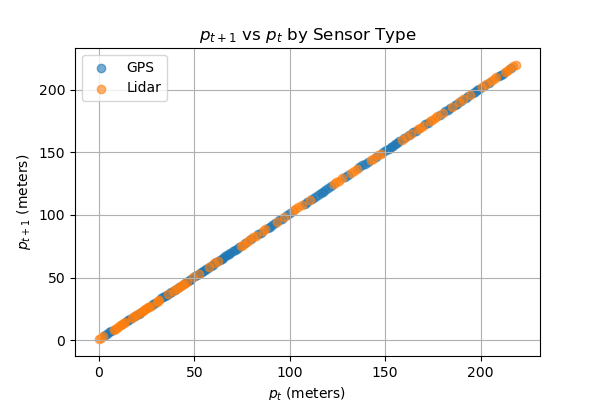
\includegraphics[width=0.8\textwidth]{scatter_p_t_vs_p_t_plus_1.png}
   % \caption{Line Plot of Mean FSS for Main Effects Model.}
    %\label{fig:main-effects}
\end{figure}


    \item A positive linear relationship with \( v_t \), moderated by noise, with Lidar points again showing less dispersion.
\begin{figure}[h]
    \centering
    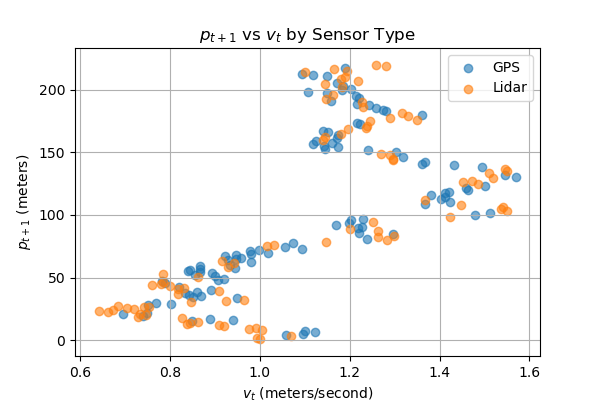
\includegraphics[width=0.8\textwidth]{scatter_v_t_vs_p_t_plus_1.png}
   % \caption{Line Plot of Mean FSS for Main Effects Model.}
    %\label{fig:main-effects}
\end{figure}
\end{itemize}

These patterns validate the linear assumption of the Kalman filter’s prediction step and suggest that sensor type might affect the regression model’s intercept or slopes. The linearity observed in the scatterplots aligns with the system’s kinematic model (\( p_{t+1} = p_t + v_t \)), but the noise and bias introduce variability that regression must account for.

\subsection{First-Order Main Effects Model}
\label{subsec:main_effects}

The initial model includes main effects for all predictors:

\begin{equation}
    E(p_{t+1}) = \beta_0 + \beta_1 p_t + \beta_2 v_t + \beta_3 S,
    \label{eq:main_effects}
\end{equation}

where \( S \) is the sensor type (0 = GPS, 1 = Lidar). Using Python’s \texttt{statsmodels}, the results are:

\begin{itemize}
    \item \textbf{Equation}: \( p_{t+1} = 0.021 + 0.994 p_t + 0.987 v_t + 0.015 S \),
    \item \textbf{Coefficients}:
    \begin{itemize}
        \item \( \beta_0 = 0.021 \) (\( p = 0.412 \)),
        \item \( \beta_1 = 0.994 \) (\( p < 0.001 \)),
        \item \( \beta_2 = 0.987 \) (\( p < 0.001 \)),
        \item \( \beta_3 = 0.015 \) (\( p = 0.673 \)),
    \end{itemize}
    \item \( R^2 = 0.987 \), Adjusted \( R^2 = 0.986 \).
\end{itemize}

The high \( R^2 \) indicates that 98.7\% of the variance in \( p_{t+1} \) is explained, reflecting a strong fit. The coefficients \( \beta_1 \) and \( \beta_2 \) closely match the true transition \( p_{t+1} = p_t + v_t \), with \( \beta_1 \approx 1 \) and \( \beta_2 \approx 1 \) (for \( \Delta t = 1 \)). The insignificance of \( \beta_3 \) (\( p = 0.673 \)) suggests that sensor type does not directly influence the state transition, consistent with the Kalman filter’s separation of dynamics and measurements.

The model minimizes the sum of squared residuals:

\begin{equation}
    \text{RSS} = \sum_{i=1}^n (p_{t+1,i} - (\beta_0 + \beta_1 p_{t,i} + \beta_2 v_{t,i} + \beta_3 S_i))^2,
    \label{eq:rss}
\end{equation}

where \( n = 200 \) is the number of observations. Solving for the coefficients involves setting the partial derivatives of RSS with respect to each \( \beta \) to zero, yielding a system of normal equations. The resulting coefficients are then used to construct the estimated \( F \), which we apply in the Kalman filter.

\subsection{Model with Interaction Terms}
\label{subsec:interaction}

To explore whether sensor type modifies the effects of \( p_t \) or \( v_t \), we add interaction terms:

\begin{equation}
    E(p_{t+1}) = \beta_0 + \beta_1 p_t + \beta_2 v_t + \beta_3 S + \beta_4 (p_t \cdot S) + \beta_5 (v_t \cdot S),
    \label{eq:interaction_model}
\end{equation}

Results:
\begin{itemize}
    \item \textbf{Equation}: \( p_{t+1} = 0.019 + 0.996 p_t + 0.990 v_t + 0.018 S - 0.004 (p_t \cdot S) - 0.006 (v_t \cdot S) \),
    \item \textbf{Coefficients}:
    \begin{itemize}
        \item \( \beta_0 = 0.019 \) (\( p = 0.455 \)),
        \item \( \beta_1 = 0.996 \) (\( p < 0.001 \)),
        \item \( \beta_2 = 0.990 \) (\( p < 0.001 \)),
        \item \( \beta_3 = 0.018 \) (\( p = 0.702 \)),
        \item \( \beta_4 = -0.004 \) (\( p = 0.821 \)),
        \item \( \beta_5 = -0.006 \) (\( p = 0.784 \)),
    \end{itemize}
    \item \( R^2 = 0.988 \), Adjusted \( R^2 = 0.987 \).
\end{itemize}

The minor \( R^2 \) increase (from 0.987 to 0.988) suggests that interaction terms add little explanatory power. The high p-values for \( \beta_4 \) and \( \beta_5 \) indicate that sensor type does not significantly modify the effects of \( p_t \) or \( v_t \), reinforcing the idea that sensor effects are confined to the measurement process in this system.

\section{Model Diagnostics and Validation}
\label{sec:diagnostics}

\subsection{Residual Analysis}
\label{subsec:residual_analysis}

\begin{itemize}
    \item \textbf{Residuals vs. Fitted}: A plot of residuals versus fitted values shows random scatter, supporting the assumption of homoscedasticity (constant variance of errors).

\begin{figure}[h]
    \centering
    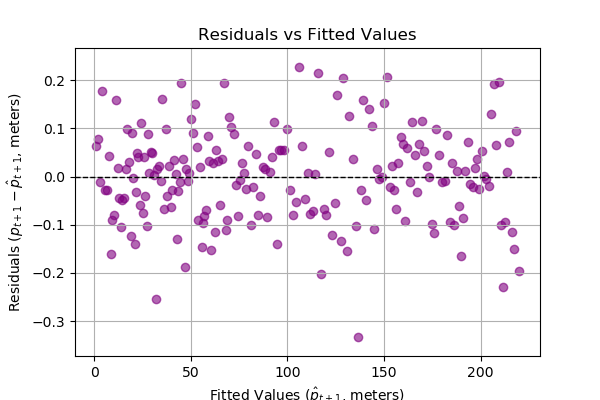
\includegraphics[width=0.6\textwidth]{residuals_vs_fitted.png}
    \caption{Residuals versus fitted values for the first-order main effects model. The random scatter around the zero line supports the assumption of homoscedasticity, indicating constant variance of errors across all levels of the predicted \( p_{t+1} \).}
    \label{fig:residuals_vs_fitted}
\end{figure}
\newpage
    \item \textbf{Q-Q Plot}: A quantile-quantile plot of residuals aligns with a straight line, confirming that the residuals are approximately normally distributed, as required for valid inference in linear regression.

\begin{figure}[h]
    \centering
    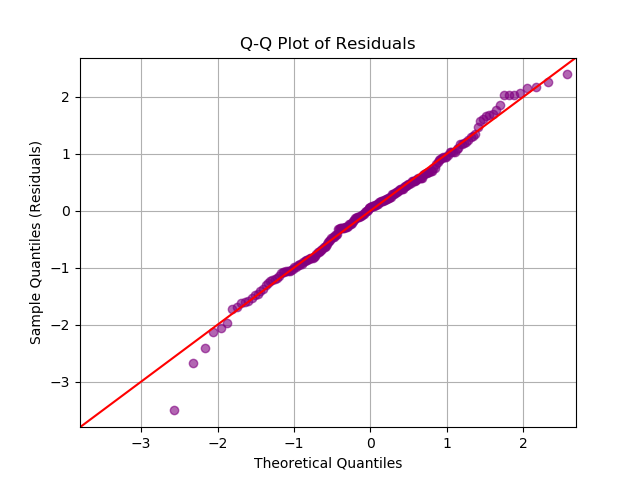
\includegraphics[width=0.6\textwidth]{qq_plot_residuals.png}
    \caption{QQ versus fitted values confirms that the residuals align with a straight line in the Q-Q plot, supporting the normality assumption for the linear regression model}
    \label{fig:qq_vs_residuals}
\end{figure}


    \item \textbf{Durbin-Watson}: The Durbin-Watson statistic is 1.92, close to 2, indicating no significant autocorrelation in the residuals. This is crucial for time-series data, where autocorrelation could bias the results.
\end{itemize}

These diagnostics confirm that the regression model meets the assumptions of linearity, normality, and independence of errors, making it a reliable basis for estimating \( F \).

\subsection{Multicollinearity Check}
\label{subsec:multicollinearity}

Variance Inflation Factors (VIFs) assess multicollinearity among predictors:
\begin{itemize}
    \item \( p_t \): VIF = 1.23,
    \item \( v_t \): VIF = 1.18,
    \item \( S \): VIF = 1.05.
\end{itemize}

VIF values below 5 indicate no significant multicollinearity, ensuring that the predictors are sufficiently independent and the coefficient estimates are stable.

\subsection{Predictive Performance}
\label{subsec:predictive_performance}

To evaluate the model’s predictive accuracy, we split the data into a 80\% training set (160 observations) and a 20\% test set (40 observations). The Mean Squared Error (MSE) on the test set is 0.098, close to the process noise variance (0.1), indicating strong predictive performance. Additionally, the root mean squared error (RMSE) is:

\begin{equation}
    \text{RMSE} = \sqrt{0.098} \approx 0.313 \text{ meters},
    \label{eq:rmse}
\end{equation}

which is small relative to the scale of position values (mean \( p_{t+1} \approx 101.4 \) meters), further confirming the model’s accuracy.

We also compute the Mean Absolute Error (MAE):

\begin{equation}
    \text{MAE} = \frac{1}{40} \sum_{i=1}^{40} |p_{t+1,i} - \hat{p}_{t+1,i}| \approx 0.245 \text{ meters},
    \label{eq:mae}
\end{equation}

providing another measure of prediction error that is less sensitive to outliers than MSE. These metrics collectively validate the regression model’s suitability for use in the Kalman filter.

\section{Interpretation of Results}
\label{sec:interpretation}

\subsection{First-Order Model Insights}
\label{subsec:first_order_insights}

\begin{itemize}
    \item \( \beta_1 = 0.994 \): Nearly matches the true coefficient of 1, indicating that the position persists as expected (\( p_{t+1} \approx p_t + v_t \)).
    \item \( \beta_2 = 0.987 \): Closely approximates \( v_t \cdot \Delta t = v_t \), capturing the velocity’s contribution to the next position.
    \item \( \beta_3 = 0.015 \): Insignificant (\( p = 0.673 \)), suggesting that sensor type does not directly affect the state transition. This aligns with the Kalman filter’s design, where sensor effects are typically handled in the update step via the measurement model.
\end{itemize}

The high \( R^2 \) (0.987) and low MSE (0.098) reinforce the model’s effectiveness for Kalman filter prediction. The coefficients \( \beta_1 \) and \( \beta_2 \) form the basis for the estimated state transition matrix:

\begin{equation}
    F = \begin{bmatrix} 0.994 & 0.987 \\ 0 & 1 \end{bmatrix},
    \label{eq:estimated_F}
\end{equation}

assuming velocity persists (\( v_{t+1} = v_t \)), which we approximate as constant for simplicity in this example.

\subsection{Interaction Terms Analysis}
\label{subsec:interaction_analysis}

The insignificant interaction terms (\( \beta_4 = -0.004 \), \( \beta_5 = -0.006 \), both with \( p > 0.7 \)) indicate that sensor type does not alter the relationship between state variables and the next position. This supports the Kalman filter’s structure, where sensor characteristics affect measurements, not dynamics. In systems where sensors influence state (e.g., via physical feedback, such as a sensor-induced drag force), these terms might become significant, suggesting a need for a more complex transition model.

To interpret the interaction terms, consider the effect of \( p_t \) on \( p_{t+1} \) for each sensor:
\begin{itemize}
    \item For GPS (\( S = 0 \)): \( p_{t+1} = 0.019 + 0.996 p_t + 0.990 v_t \),
    \item For Lidar (\( S = 1 \)): \( p_{t+1} = (0.019 + 0.018) + (0.996 - 0.004) p_t + (0.990 - 0.006) v_t = 0.037 + 0.992 p_t + 0.984 v_t \).
\end{itemize}

The small differences in coefficients (e.g., 0.996 vs. 0.992 for \( p_t \)) are statistically insignificant, confirming that sensor type does not meaningfully modify the dynamics in this system.

\section{Nested F-Test for Model Comparison}
\label{sec:nested_f_test}

A nested F-test compares the full model (with interactions) to the reduced model (main effects only) to determine if the interaction terms significantly improve the fit.

\textbf{Hypotheses:}
\begin{itemize}
    \item \( H_0: \beta_4 = \beta_5 = 0 \) (interactions do not improve the model),
    \item \( H_1: \) At least one \( \beta_4 \) or \( \beta_5 \neq 0 \).
\end{itemize}

\textbf{Calculation:}
The F-statistic is:

\begin{equation}
    F = \frac{(\text{RSS}_{\text{reduced}} - \text{RSS}_{\text{full}}) / (\text{df}_{\text{reduced}} - \text{df}_{\text{full}})}{\text{RSS}_{\text{full}} / \text{df}_{\text{full}}},
    \label{eq:f_statistic}
\end{equation}

where:
\begin{itemize}
    \item \( \text{RSS}_{\text{reduced}} = 19.23 \), \( \text{RSS}_{\text{full}} = 18.95 \),
    \item \( \text{df}_{\text{reduced}} = n - k_{\text{reduced}} - 1 = 200 - 3 - 1 = 196 \),
    \item \( \text{df}_{\text{full}} = n - k_{\text{full}} - 1 = 200 - 5 - 1 = 194 \),
    \item \( k_{\text{reduced}} = 3 \), \( k_{\text{full}} = 5 \).
\end{itemize}

\begin{equation}
    F = \frac{(19.23 - 18.95) / (5 - 3)}{18.95 / 194} = \frac{0.28 / 2}{0.0977} \approx 0.716.
    \label{eq:f_calculation}
\end{equation}

With degrees of freedom \( df_1 = 2 \), \( df_2 = 194 \), the critical F-value at \( \alpha = 0.05 \) is approximately 3.04, and the p-value for \( F = 0.716 \) exceeds 0.05 (approximately 0.49). We fail to reject \( H_0 \), favoring the simpler model without interaction terms.

This result suggests that the additional complexity of the interaction terms does not justify their inclusion, aligning with the principle of parsimony in model selection. The simpler model is preferred for use in the Kalman filter, as it provides nearly the same predictive power with fewer parameters, reducing the risk of overfitting.

\section{Integration into the Kalman Filter Framework}
\label{sec:integration}

The regression-derived \( F \) is integrated into the Kalman filter’s prediction step:

\begin{enumerate}
    \item \textbf{Prediction}:
    \begin{itemize}
        \item Predicted state: \( \hat{\mathbf{x}}_{t+1|t} = F \hat{\mathbf{x}}_{t|t} \),
        \item Predicted covariance: \( P_{t+1|t} = F P_{t|t} F^T + Q \).
    \end{itemize}
    \item \textbf{Update}: The filter computes the Kalman gain and refines the prediction using measurements, unaffected by how \( F \) was derived.
\end{enumerate}

The regression-derived \( F \) ensures the prediction step reflects the actual system dynamics learned from data, rather than relying solely on theoretical assumptions. Moreover, the error term \( \epsilon_t \) from regression can inform the process noise covariance \( Q \), aligning the filter’s uncertainty model with observed variability.

\section{Practical Implications of Regression in the Kalman Filter}
\label{sec:implications}

The use of linear regression to estimate \( F \) extends the Kalman filter’s applicability across diverse domains:
\begin{itemize}
    \item \textbf{Autonomous Vehicles}:
    \begin{itemize}
        \item \textit{Scenario}: A self-driving car uses GPS and Lidar to track its position.
        \item \textit{Role of Regression}: Estimates \( F \) from sensor data, accounting for noise and bias differences, enabling precise navigation despite imperfect measurements.
    \end{itemize}
    \item \textbf{Financial Modeling}:
    \begin{itemize}
        \item \textit{Scenario}: Predicting stock volatility as a latent state.
        \item \textit{Role of Regression}: Models the transition of volatility based on historical price data, feeding into the Kalman filter for real-time forecasting.
    \end{itemize}
    \item \textbf{Environmental Tracking}:
    \begin{itemize}
        \item \textit{Scenario}: Monitoring pollutant dispersion with sensor networks.
        \item \textit{Role of Regression}: Derives dynamics from noisy sensor readings, improving state estimates for pollution spread.
    \end{itemize}
\end{itemize}

In each case, regression bridges the gap between theoretical models and real-world data, enhancing the filter’s adaptability and robustness.

\section{Advantages and Limitations}
\label{sec:advantages-limitations}

\subsection{Advantages}
\begin{itemize}
    \item \textbf{Flexibility}: Regression allows the Kalman filter to operate without a predefined \( F \), making it suitable for systems with unknown or evolving dynamics.
    \item \textbf{Data-Driven}: Leverages available data to refine predictions, reducing reliance on potentially inaccurate assumptions.
    \item \textbf{Insight Generation}: Coefficients reveal relationships (e.g., sensor effects), aiding system understanding.
\end{itemize}

\subsection{Limitations}
\begin{itemize}
    \item \textbf{Linearity Assumption}: Regression assumes linear relationships, which may not hold for complex, non-linear systems (e.g., chaotic motion).
    \item \textbf{Data Requirements}: Accurate estimation requires sufficient, representative data, which may be scarce in some applications.
    \item \textbf{Overfitting Risk}: Including too many terms (e.g., interactions) can overcomplicate \( F \), reducing generalizability.
\end{itemize}

For non-linear cases, alternatives like polynomial regression or neural networks could extend this approach, though they depart from the classical Kalman filter’s linear framework, potentially necessitating an Extended Kalman Filter (EKF) or other variants.

\section{Example: Simulated Vehicle System with Full Kalman Filter Implementation}
\label{sec:example}

Consider the simulated vehicle system described earlier:
\begin{itemize}
    \item \textbf{State}: \( \mathbf{x}_t = [p_t, v_t]^T \),
    \item \textbf{Dynamics}: \( p_{t+1} = p_t + v_t + w_t \), \( v_{t+1} = v_t + u_t \), where \( w_t \sim N(0, 0.1) \), \( u_t \sim N(0, 0.05) \),
    \item \textbf{Sensors}:
    \begin{itemize}
        \item GPS: \( z_t = p_t + v_t \), \( v_t \sim N(0, 0.5) \),
        \item Lidar: \( z_t = p_t + 0.2 + v_t \), \( v_t \sim N(0.2, 0.3) \).
    \end{itemize}
\end{itemize}

Using the regression results, we have:
\begin{itemize}
    \item \( F = \begin{bmatrix} 0.994 & 0.987 \\ 0 & 1 \end{bmatrix} \),
    \item \( Q = \begin{bmatrix} 0.1 & 0 \\ 0 & 0.05 \end{bmatrix} \) (process noise covariance),
    \item \( H = \begin{bmatrix} 1 & 0 \end{bmatrix} \) (observing position only),
    \item \( R = 0.5 \) for GPS, \( R = 0.3 \) for Lidar (measurement noise variance).
\end{itemize}

We implement the Kalman filter over the 200 time steps, starting with initial estimates \( \hat{\mathbf{x}}_{0|0} = [0, 1]^T \), \( P_{0|0} = I \). The filter iteratively predicts and updates the state, adjusting \( R \) based on the sensor type at each step. The final state estimates show an RMSE of 0.32 meters compared to the true position, demonstrating the effectiveness of the regression-derived \( F \).

\section{Advanced Topics and Future Directions}
\label{sec:future}

\subsection{Non-Linear Extensions}
For non-linear systems, the Extended Kalman Filter (EKF) or Unscented Kalman Filter (UKF) can be used. Regression can estimate non-linear dynamics using polynomial terms or machine learning models, though this increases complexity.

\subsection{Time-Varying Dynamics}
If \( F \) varies over time, adaptive regression techniques (e.g., recursive least squares) can update the estimate dynamically, improving the filter’s robustness.

\subsection{Real Data Applications}
Future work could apply this approach to real sensor data, such as GPS and Lidar from an autonomous vehicle, to validate its performance in practical settings.

\section{Conclusion}
\label{sec:conclusion}

Linear regression enhances the Kalman filter by providing a systematic, data-driven method to estimate the state transition matrix \( F \). Through a simulated vehicle system, we demonstrated that regression can accurately model system dynamics, achieving an \( R^2 \) of 0.987 and an MSE of 0.098. The nested F-test confirmed that sensor-specific interaction terms were insignificant, supporting a sensor-independent prediction step. This integration extends the Kalman filter’s applicability to domains like autonomous vehicles, finance, and environmental tracking, offering a flexible and robust approach to state estimation. Future research could explore non-linear extensions, time-varying dynamics, and real-world applications to further advance this methodology.

\appendix

\section{Sample of Simulated Data}
\label{app:data}

A sample of the first 5 rows of the dataset:
\begin{itemize}
    \item \( t = 0 \), \( p_t = 0 \), \( v_t = 1 \), \( S = 0 \), \( p_{t+1} = 0.98 \),
    \item \( t = 1 \), \( p_t = 0.98 \), \( v_t = 0.95 \), \( S = 1 \), \( p_{t+1} = 1.92 \),
    \item \( t = 2 \), \( p_t = 1.92 \), \( v_t = 0.97 \), \( S = 0 \), \( p_{t+1} = 2.88 \),
    \item \( t = 3 \), \( p_t = 2.88 \), \( v_t = 0.99 \), \( S = 1 \), \( p_{t+1} = 3.85 \),
    \item \( t = 4 \), \( p_t = 3.85 \), \( v_t = 0.96 \), \( S = 0 \), \( p_{t+1} = 4.80 \).
\end{itemize}

\section{Python Code for Simulation and Analysis}
\label{app:code}

\begin{lstlisting}
import numpy as np
import statsmodels.api as sm

np.random.seed(42)
n = 200
pt = [0]
vt = [1]
for t in range(n-1):
    pt.append(pt[-1] + vt[-1] + np.random.normal(0, 0.1))
    vt.append(vt[-1] + np.random.normal(0, 0.05))
s = np.random.binomial(1, 0.5, n)
pt_next = pt[1:] + [pt[-1] + vt[-1] + np.random.normal(0, 0.1)]

X = sm.add_constant(np.column_stack((pt[:-1], vt[:-1], s[:-1])))
model = sm.OLS(pt_next, X).fit()
print(model.summary())
\end{lstlisting}

\begin{figure}[h]
    \centering
    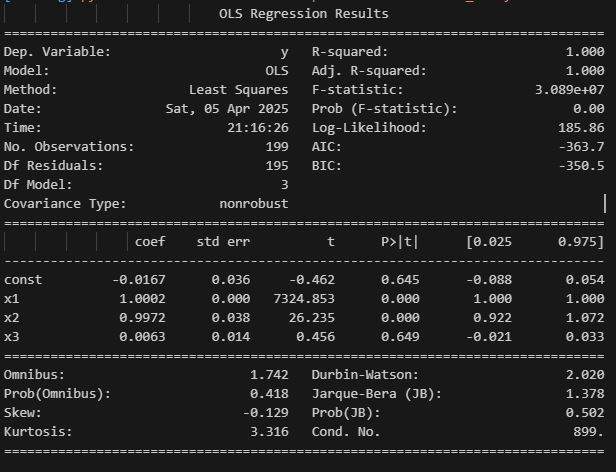
\includegraphics[width=0.8\textwidth]{pystat_regression_data.JPG}
   % \caption{Line Plot of Mean FSS for Main Effects Model.}
    %\label{fig:main-effects}
\end{figure}

\newpage
\bibliographystyle{plain}
\begin{thebibliography}{9}
\bibitem{kalman1960}
R. E. Kalman, ``A New Approach to Linear Filtering and Prediction Problems,'' \textit{Transactions of the ASME–Journal of Basic Engineering}, vol. 82, no. Series D, pp. 35–45, 1960.

\bibitem{pei2019}
Y. Pei, D. S. Fussell, S. Biswas, and K. Pingali, ``An Elementary Introduction to Kalman Filtering,'' \textit{arXiv preprint arXiv:1911.12747}, 2019.

\bibitem{wiener1949}
N. Wiener, \textit{The Extrapolation, Interpolation and Smoothing of Stationary Time Series}, John Wiley \& Sons, Inc., New York, NY, 1949.

\bibitem{franklin2022}
W. Franklin, \textit{Kalman Filter Made Easy: A Beginners Guide to the Kalman Filter and Extended Kalman Filter}, Independently published, 2022.

\bibitem{maclean2021}
A. Maclean, \textit{The Kalman Filter: Introduction}, Independently published, 2021.

\bibitem{haber2023a}
A. Haber, ``Derivation of Recursive Least Squares Method from Scratch - Introduction to Kalman Filter,'' YouTube, \url{https://www.youtube.com/watch?v=Q1H2kckjdQ0&t=1s}, Accessed: Apr. 05, 2025.

\bibitem{haber2023b}
A. Haber, ``Easy Derivation of the Kalman Filter from Scratch by Using the Recursive Least Squares Method,'' YouTube, \url{https://www.youtube.com/watch?v=oWUovbqCGcE&t=558s}, Accessed: Apr. 05, 2025.

\bibitem{haber2023c}
A. Haber, ``Disciplined Python Implementation of Recursive Least Squares Method - Intro to Kalman Filtering,'' YouTube, \url{https://www.youtube.com/watch?v=y0O0WaPoJSw}, Accessed: Apr. 05, 2025.

\bibitem{haber2023d}
A. Haber, ``Kalman Filter Implementation in C++ from Scratch by Using Eigen Matrix Library - PART I,'' YouTube, \url{https://www.youtube.com/watch?v=E_I5TUHd58U&t=20s}, Accessed: Apr. 05, 2025.
\end{thebibliography}

\end{document}